\documentclass[svgnames, border=0.3mm]{standalone}
\usepackage{tikz}
\usepackage{xcolor}
% \usepackage{xfp} % Uncomment this line if you encounter a problem with \inteval{} expression
\usetikzlibrary{calc,math,shadows,arrows.meta,decorations.markings}
\newenvironment{standalonepage}{}{} %Dummy environment that contains pictures in the same page
\standaloneenv{standalonepage} %The dummy environment is make known to the stand alone class

\begin{document}
\begin{standalonepage}
    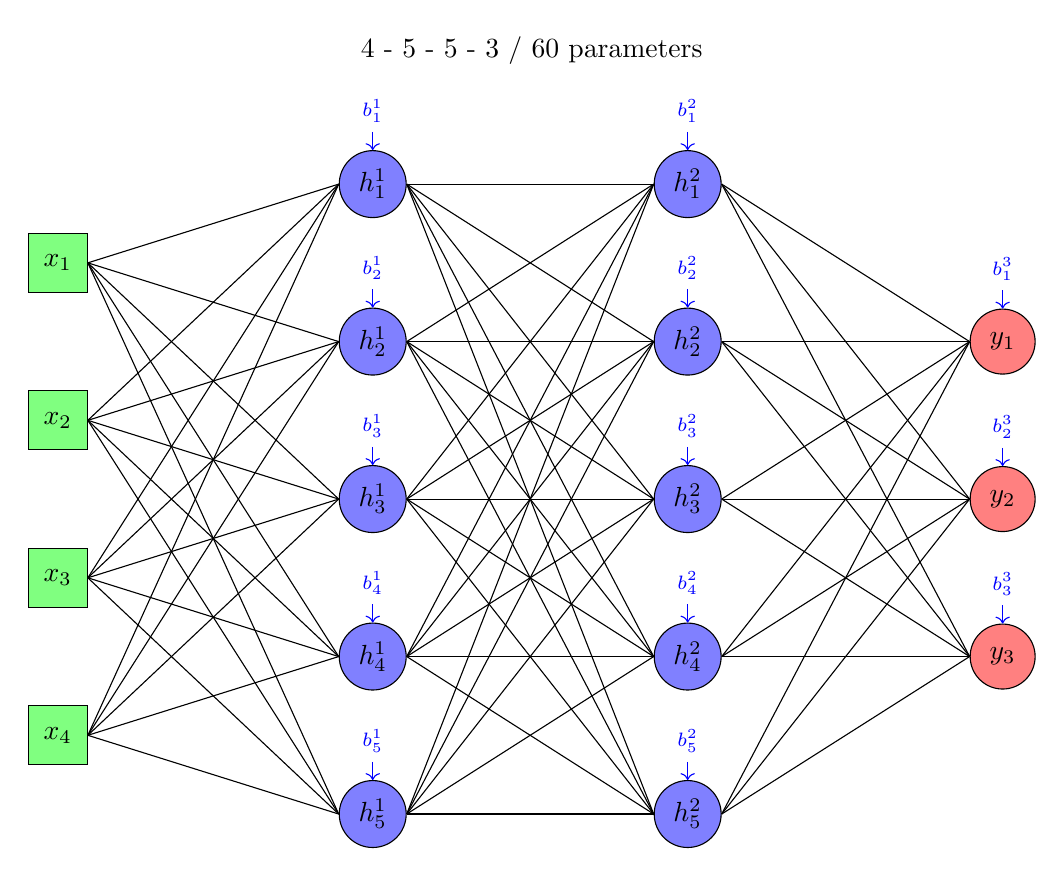
\begin{tikzpicture}[
        input/.style={rectangle, draw, minimum size=.75cm, fill=green!50},
        neuron/.style={circle, draw, minimum size=.825cm},
        hidden neuron/.style={neuron, fill=blue!50},
        output neuron/.style={neuron, fill=red!50},
        bias/.style={font=\scriptsize, text=blue},
        weight/.style={above, sloped, font=\tiny, yshift=-0.1cm, pos=0.15},
        positive weight/.style={weight, draw=green!50!black},
        negative weight/.style={weight, draw=red!75},
        false negative weight/.style={weight, draw=Orchid!75},
        unsigned weight/.style={weight, draw=black}
    ]

        % Define the network architecture as an array
        % Each element represents the number of neurons in that layer
        \def\networkShape{4,5,5,3}

        % Weights signs
        \def\positiveWeights{}
        \def\negativeWeights{}
        \def\falseNegativeWeights{}

        % Values of all model weights
        \def\weightValues{}
        \def\biasValues{{0.1, 0.2, 0.15, 0.25, 0.3}, {0.05, 0.1, 0.15, 0.2, 0.25}, {0.1, 0.4, 0.35}}

        % Display the index number or not (0 no / 1 yes)
        \pgfmathsetmacro{\displayIndex}{0}

        % Display bias on each neurons
        \pgfmathsetmacro{\displayBias}{1}
        \pgfmathsetmacro{\displayBiasValue}{0} % if set to 0, a name will be given instead of the value

        % Extract the number of layers
        \pgfmathsetmacro{\numLayers}{dim({\networkShape})-1}
        \pgfmathsetmacro{\numInputs}{{\networkShape}[0]}
        \pgfmathsetmacro{\numFirstHiddenLayer}{{\networkShape}[1]}
        \pgfmathsetmacro{\numOutputs}{{\networkShape}[\numLayers]}
        \pgfmathsetmacro{\inputOffset}{(\numInputs - 1) / 2}

        % Input neurons
        \foreach \i in {1,...,\numInputs} {
            \node[input] (x\i) at (0, -\i*2 + \inputOffset*2 + 2) {$x_{\i}$};
        }

        % Hidden layers
        \pgfmathsetmacro{\numHiddenLayers}{{\numLayers - 1}}
        \foreach \layer in {1,...,\numHiddenLayers} {
            \pgfmathsetmacro{\numNeurons}{{\networkShape}[\layer]}
            \pgfmathsetmacro{\offset}{(\numNeurons - 1) / 2}
            \foreach \i in {1,...,\numNeurons} {
                \node[hidden neuron] (h\layer\i) at (4*\layer, -\i*2 + \offset*2 + 2) {$h^{\layer}_{\i}$};
                \ifnum\displayBias=1
                    \ifnum\displayBiasValue=1
                        \node[bias] (bias\layer\i) at ([yshift=5mm]h\layer\i.north) {\pgfmathparse{{\biasValues}[\layer-1][\i-1]}\pgfmathresult};
                    \else
                        \node[bias] (bias\layer\i) at ([yshift=5mm]h\layer\i.north) {$b^{\layer}_{\i}$};
                    \fi
                    \draw[->, blue] (bias\layer\i) -- (h\layer\i);
                \fi
            }
        }

        % Output neurons
        \pgfmathsetmacro{\outputOffset}{(\numOutputs - 1) / 2}
        \pgfmathsetmacro{\lastLayer}{int(\numLayers)}
        \foreach \i in {1,...,\numOutputs} {
            \node[output neuron] (y\i) at (4*\numLayers, -\i*2 + \outputOffset*2 + 2) {$y_{\i}$};
            \ifnum\displayBias=1
                \ifnum\displayBiasValue=1
                    \node[bias] (bias\i) at ([yshift=5mm]y\i.north) {\pgfmathparse{{\biasValues}[\numHiddenLayers][\i-1]}\pgfmathresult};
                \else
                    \node[bias] (bias\i) at ([yshift=5mm]y\i.north) {$b^{\lastLayer}_{\i}$};
                \fi
                \draw[->, blue] (bias\i) -- (y\i);
            \fi
        }

        % Connections with weights from inputs to first layer
        \foreach \i in {1,...,\numInputs} {
            \foreach \j in {1,...,\numFirstHiddenLayer} {
                \pgfmathsetmacro{\index}{int((\i-1)*\numFirstHiddenLayer + \j - 1)}
                % Check if the index is in positive, negative or false negative weights
                \pgfmathsetmacro{\isPositive}{0}
                \pgfmathsetmacro{\isNegative}{0}
                \pgfmathsetmacro{\isFalseNegative}{0}
                \foreach \k in \positiveWeights {
                    \pgfmathparse{int(\k == \index ? 1 : \isPositive)}
                    \global\let\isPositive\pgfmathresult
                }
                \foreach \k in \negativeWeights {
                    \pgfmathparse{int(\k == \index ? 1 : \isNegative)}
                    \global\let\isNegative\pgfmathresult
                }
                \foreach \k in \falseNegativeWeights {
                    \pgfmathparse{int(\k == \index ? 1 : \isFalseNegative)}
                    \global\let\isFalseNegative\pgfmathresult
                }
                % \pgfmathsetmacro{\getValue}{{\weightValues}[\index]}
                \ifnum\isPositive=1
                    \ifnum\displayIndex=1
                        \draw[positive weight] (x\i.east) -- (h1\j.west) node[weight] {\index};
                    \else
                        \draw[positive weight] (x\i.east) -- (h1\j.west) node[weight] {};
                    \fi
                \else
                    \ifnum\isNegative=1
                        \ifnum\displayIndex=1
                            \draw[negative weight] (x\i.east) -- (h1\j.west) node[weight] {\index};
                        \else
                            \draw[negative weight] (x\i.east) -- (h1\j.west) node[weight] {};
                        \fi
                    \else
                        \ifnum\isFalseNegative=1
                            \ifnum\displayIndex=1
                                \draw[false negative weight] (x\i.east) -- (h1\j.west) node[weight] {\index};
                            \else
                                \draw[false negative weight] (x\i.east) -- (h1\j.west) node[weight] {};
                            \fi
                        \else
                            \ifnum\displayIndex=1
                                \draw[unsigned weight] (x\i.east) -- (h1\j.west) node[weight] {\index};
                            \else
                                \draw[unsigned weight] (x\i.east) -- (h1\j.west) node[weight] {};
                            \fi
                        \fi
                    \fi
                \fi
            }
        }

        % Connections with weights first hidden layer to last hidden layer
        \pgfmathsetmacro{\lastHiddenLayer}{int(\numHiddenLayers-1)}
        \newcounter{indexCounter}
        \pgfmathtruncatemacro{\startIndex}{\numInputs * \numFirstHiddenLayer}
        \setcounter{indexCounter}{\startIndex}
        \ifnum\lastHiddenLayer>0
            \foreach \layer in {1,...,\lastHiddenLayer} {
                \pgfmathsetmacro{\numNeuronsCurrent}{{\networkShape}[\layer]}
                \pgfmathsetmacro{\numNeuronsNext}{{\networkShape}[\layer+1]}
                \foreach \i in {1,...,\numNeuronsCurrent} {
                    \foreach \j in {1,...,\numNeuronsNext} {
                        % Use the global counter instead of recalculating
                        \pgfmathsetmacro{\index}{\value{indexCounter}}
                        % Check if the index is in positive, negative or false negative weights
                        \pgfmathsetmacro{\isPositive}{0}
                        \pgfmathsetmacro{\isNegative}{0}
                        \pgfmathsetmacro{\isFalseNegative}{0}
                        \foreach \k in \positiveWeights {
                            \pgfmathparse{int(\k == \index ? 1 : \isPositive)}
                            \global\let\isPositive\pgfmathresult
                        }
                        \foreach \k in \negativeWeights {
                            \pgfmathparse{int(\k == \index ? 1 : \isNegative)}
                            \global\let\isNegative\pgfmathresult
                        }
                        \foreach \k in \falseNegativeWeights {
                            \pgfmathparse{int(\k == \index ? 1 : \isFalseNegative)}
                            \global\let\isFalseNegative\pgfmathresult
                        }
                        % \pgfmathsetmacro{\getValue}{{\weightValues}[\index]}
                        \ifnum\isPositive=1
                            \ifnum\displayIndex=1
                                \draw[positive weight] (h\layer\i.east) -- (h\inteval{\layer+1}\j.west) node[weight] {\index};
                            \else
                                \draw[positive weight] (h\layer\i.east) -- (h\inteval{\layer+1}\j.west) node[weight] {};
                            \fi
                        \else
                            \ifnum\isNegative=1
                                \ifnum\displayIndex=1
                                    \draw[negative weight] (h\layer\i.east) -- (h\inteval{\layer+1}\j.west) node[weight] {\index};
                                \else
                                    \draw[negative weight] (h\layer\i.east) -- (h\inteval{\layer+1}\j.west) node[weight] {};
                                \fi
                            \else
                                \ifnum\isFalseNegative=1
                                    \ifnum\displayIndex=1
                                        \draw[false negative weight] (h\layer\i.east) -- (h\inteval{\layer+1}\j.west) node[weight] {\index};
                                    \else
                                        \draw[false negative weight] (h\layer\i.east) -- (h\inteval{\layer+1}\j.west) node[weight] {};
                                    \fi
                                \else
                                    \ifnum\displayIndex=1
                                        \draw[unsigned weight] (h\layer\i.east) -- (h\inteval{\layer+1}\j.west) node[weight] {\index};
                                    \else
                                        \draw[unsigned weight] (h\layer\i.east) -- (h\inteval{\layer+1}\j.west) node[weight] {};
                                    \fi
                                \fi
                            \fi
                        \fi
                        % Increment the global index counter
                        \addtocounter{indexCounter}{1}
                    }
                }
            }
        \fi

        \pgfmathsetmacro{\lastHiddenLayer}{int(\numLayers - 1)}
        \pgfmathsetmacro{\numNeurons}{{\networkShape}[\lastHiddenLayer]}
        \foreach \i in {1,...,\numNeurons}{
            \foreach \k in {1,...,\numOutputs} {
                % Use the global counter instead of recalculating
                \pgfmathsetmacro{\index}{\value{indexCounter}}
                % Check if the index is in positive, negative or false negative weights
                \pgfmathsetmacro{\isPositive}{0}
                \pgfmathsetmacro{\isNegative}{0}
                \pgfmathsetmacro{\isFalseNegative}{0}
                \foreach \k in \positiveWeights {
                    \pgfmathparse{int(\k == \index ? 1 : \isPositive)}
                    \global\let\isPositive\pgfmathresult
                }
                \foreach \k in \negativeWeights {
                    \pgfmathparse{int(\k == \index ? 1 : \isNegative)}
                    \global\let\isNegative\pgfmathresult
                }
                \foreach \k in \falseNegativeWeights {
                    \pgfmathparse{int(\k == \index ? 1 : \isFalseNegative)}
                    \global\let\isFalseNegative\pgfmathresult
                }
                % \pgfmathsetmacro{\getValue}{{\weightValues}[\index]}
                \ifnum\isPositive=1
                    \ifnum\displayIndex=1
                        \draw[positive weight] (h\lastHiddenLayer\i.east) -- (y\k.west) node[weight] {\index};
                    \else
                        \draw[positive weight] (h\lastHiddenLayer\i.east) -- (y\k.west) node[weight] {};
                    \fi
                \else
                    \ifnum\isNegative=1
                        \ifnum\displayIndex=1
                            \draw[negative weight] (h\lastHiddenLayer\i.east) -- (y\k.west) node[weight] {\index};
                        \else
                            \draw[negative weight] (h\lastHiddenLayer\i.east) -- (y\k.west) node[weight] {};
                        \fi
                    \else
                        \ifnum\isFalseNegative=1
                            \ifnum\displayIndex=1
                                \draw[false negative weight] (h\lastHiddenLayer\i.east) -- (y\k.west) node[weight] {\index};
                            \else
                                \draw[false negative weight] (h\lastHiddenLayer\i.east) -- (y\k.west) node[weight] {};
                            \fi
                        \else
                            \ifnum\displayIndex=1
                                \draw[unsigned weight] (h\lastHiddenLayer\i.east) -- (y\k.west) node[weight] {\index};
                            \else
                                \draw[unsigned weight] (h\lastHiddenLayer\i.east) -- (y\k.west) node[weight] {};
                            \fi
                        \fi
                    \fi
                \fi
                % Increment the global index counter
                \addtocounter{indexCounter}{1}
            }
        }

        % Display network shape as text
        \pgfmathsetmacro{\nbLayers}{int(\numLayers)}
        \pgfmathsetmacro{\index}{\value{indexCounter}}
        \def\networkText{}
        \foreach \i in {0,...,\nbLayers} {
                \pgfmathparse{{\networkShape}[\i]}
                \xdef\networkText{\networkText\pgfmathresult}
                \ifnum\i<\nbLayers
                    \xdef\networkText{\networkText~- }
                \fi
            }
        \node (text) at ($(current bounding box.north) + (0,.5)$) {%
            \networkText~/ \index~parameters
        };

        % Or display specific title at the center of the figure
        % \node (text) at ($(current bounding box.north) + (0,.5)$) {Example};
    \end{tikzpicture}
\end{standalonepage}
\end{document}
